%%%%%%%%%%%%%%%%%%%%%%%%%%%%%%%%%%%%%%%%%%%%%%%%%%%%%%%%%%
%%
%% MARK: Title
%%
%%%%%%%%%%%%%%%%%%%%%%%%%%%%%%%%%%%%%%%%%%%%%%%%%%%%%%%%%%

\chapter*{\S B7. Differential of Holonomy for Torus Bundles}
\setcounter{footnote}{0}

%%%%%%%%%%%%%%%%%%%%%%%%%%%%%%%%%%%%%%%%%%%%%%%%%%%%%%%%%%
%%
%% MARK: Abstract
%%
%%%%%%%%%%%%%%%%%%%%%%%%%%%%%%%%%%%%%%%%%%%%%%%%%%%%%%%%%%

\begin{abstract}
  We make explicit the holonomy function on a torus bundle over a diffeological space.
  Here the word torus denotes any quotient $\Torus=\RR/\Gamma$,
  where $\Gamma$ is a strict subgroup of $\RR$.
  Then,
  we give an explicit formula for the differential of the holonomy in terms of the Chain-Homotopy Operator and the curvature.
\end{abstract}

In this note we will consider a principal fiber bundle $\pi : Y \to X$,
with $X$ and $Y$ two diffeological spaces,
and with structure group a \emph{torus} $\Torus = \RR/\Gamma$,
where $\Gamma$ is any strict subgroup of $\RR$.
As we know,
if $\Gamma = a \ZZ$ then the torus $\Torus$ is a manifold isomorphic to the circle $\Sph^1$,
and if $\Gamma$ has more than one generator,
$\Torus$ is said to be \emph{irrational},
and it is no longer a manifold.
We assume that there exists on $Y$ a connection form $\lambda$,
that is,
a differential $1$-form satisfying the two conditions
\begin{enumerate}
  \item $\lambda$ is \textbf{invariant} under the action of $\Torus$:
  $$%
    \mbox{For all $\tau \in \Torus$}, \quad \tau_Y^*(\lambda) = \lambda,
    $$%
  where $\tau_Y$ denotes the action of $\tau$ on $Y$.
  \item $\lambda$ is \textbf{calibrated}:
  $$%
    \mbox{For all $y \in Y$}, \quad \hat y^*(\lambda) = \theta,
    $$%
  where $\hat y : \Torus \to Y$ is the orbit map $\hat y(\tau) = \tau_Y(y)$,
  and $\theta$ is the canonical $1$-form on $\Torus$,
  the pushforward of the canonical $1$-form $dt$ on $\RR$.
\end{enumerate}
The connection then defines the set of \emph{horizontal paths} in $Y$:
$$%
  \mbox{Hor}(Y) = \{ \gamma \in \Paths(Y) \mid \lambda(\gamma)_t = 0 \mbox{ for all } t \in \RR \}.
  $$%
See \cite{PIZ13} for the details of these constructions,
in particular \textsection\,8.37.

%%%%%%%%%%%%%%%%%%%%%%%%%%%%%%%%%%%%%%%%%%%%%%%%%%%%%%%%%%
%%
%% MARK: Loops Bundles
%%
%%%%%%%%%%%%%%%%%%%%%%%%%%%%%%%%%%%%%%%%%%%%%%%%%%%%%%%%%%
\section{Loops bundles}

\begin{Article}{Exercise I.}{}
  Show that the pushforward
  $$%
    \pi_* : \Loops(Y) \to \Loops(X),
    \mbox{ defined by }
    \pi_*(\tilde \ell) = \pi \circ \tilde \ell,
    $$%
  is surjective.
\end{Article}

\begin{proof}
  Consider a loop $\ell$ in $X$,
  that is,
  $\ell \in \Cinfty(\RR,X)$ and $\ell(0)=\ell(1)$.
  The pullback of $Y$ by $\ell$ is a principal bundle over $\RR$ with a connection,
  therefore it is trivial \cite[\textsection\,8.34]{PIZ13}:
  there exists an equivariant diffeomorphism $\pphi:\RR\times \Torus \to \ell^*(Y)$.
  Write $\pphi(t,\tau) = (t,f(t,\tau))$,
  with $f(t,\tau) \in Y_{\ell(t)}$.
  \[
  \begin{tikzcd}
    \RR \times \Torus \arrow{r}{\pphi} \arrow[swap]{dr}{\Proj_1} & \ell^*(Y) \arrow{d}{\Proj_1} \arrow{r}{\Proj_2}       & Y  \arrow{d}{\pi} \\
    & \RR \arrow{r}[swap]{\ell} & X
  \end{tikzcd}
  \]
  By equivariance,
  $\pphi(t,\tau)=(t,\tau_Y(f(t)))$,
  where $f\in \Paths(Y)$ and $\pi\circ f= \ell$.
  There exists a unique $a\in \Torus$ such that $f(1)=a_Y(f(0))$.
  Now,
  since $\Torus$ is connected there exists a path $\tau \in \Paths(\Torus)$ such that $\tau(0)=1$ and $\tau(1) = a^{-1}$.
  Then,
  $\tilde \ell: t \mapsto \tau(t)_Y(f(t))$ is a path in $Y$ such that $\pi \circ \tilde \ell = \ell$,
  and $\tilde \ell(0)=\tilde \ell(1)=f(0)$.
  Therefore,
  $\tilde \ell \in \Loops(Y)$ and $\pi \circ \tilde \ell = \ell$.
\end{proof}

Now, $\pi_*$ is not only surjective. Using the same ideas as in Exercise I:

\begin{Article}{Exercise II.}{}
  Show that the pushforward $\pi_* : \Loops(Y) \to \Loops(X)$ is not only surjective but actually a subduction.
\end{Article}

\begin{proof}
  Let $r\mapsto \ell_r$ be a plot in $\Loops(X)$ defined on a small open ball $B$ centered at $0$ in some $\RR^n$.
  Since $r\mapsto \ell_r$ is smooth,
  the map $Q : (r,t) \mapsto \ell_r(t)$ defined on $B \times \RR$ is a plot of $X$.
  Because we have a connection on $\pi : Y \to X$,
  we obtain a connection,
  by pullback,
  on $\Proj_1  : Q^*(Y) \to B \times \RR$.
  Since $B \times \RR$ is contractible,
  the fibration $\Proj_1  : Q^*(Y) \to B \times \RR$ is trivial,
  that is,
  there exists an equivariant diffeomorphism $\pphi : B \times \RR \times \Torus \to Q^*(Y)$.
  By equivariance,
  $\pphi(r,t,\tau)=(r,t,\tau_Y(f_r(t)))$,
  where $(r,t) \mapsto f_r(t)$ is a plot of $Y$.
  This is equivalent to saying that $r \mapsto f_r$ is a plot of $\Paths(Y)$.
  We then have $\pi \circ f_r(t) = \ell_r(t)$.
  \[
  \begin{tikzcd}
    B \times \RR \times \Torus \arrow{r}{\pphi} \arrow[swap]{dr}{\Proj_{1,2}} & Q^*(Y) \arrow{d}{\Proj_1} \arrow{r}{\Proj_3}       & Y  \arrow{d}{\pi} \\
    & B \times \RR \arrow{r}[swap]{Q} & X
  \end{tikzcd}
  \]
  Thus,
  there exists $r \mapsto a_r \in \Torus$ such that $f_r(1) = (a_r)_Y(f_r(0))$.
  Let $\alpha : r \mapsto f_r(0)$ and $\beta : r \mapsto f_r(1)$.
  Since $\alpha$ and $\beta$ are homotopic,
  the pullbacks $\alpha^*(Y)$ and $\beta^*(Y)$ are equivalent (in fact trivial) \cite[\textsection\,8.34]{PIZ13}.
  Therefore,
  $r\mapsto a_r$ is a plot of $\Torus$,
  as is $r\mapsto a_r^{-1}$.
  Now,
  the projection $\Class : \RR \to \Torus$ is the universal covering.
  Since the ball $B$ is contractible,
  there exists a unique lifting $r \mapsto \bar a_r$ of $r\mapsto a_r^{-1}$ such that $\bar a_0=0$ \cite[\textsection\,8.25]{PIZ13}.
  Consider then $(r,t) \mapsto \tau_r(t) = \Class(t\bar a_r)$.
  The parametrization $r \mapsto \tau_r$ is a plot of $\Paths(\Torus)$ satisfying $\tau_r(0) = 1$ and $\tau_r(1) = a_r^{-1}$.
  Then,
  define $\tilde \ell_r(t)=\tau_r(t)_Y(f_r(t))$;
  this is a plot of $Y$ such that $\tilde \ell_r(0)=f_r(0)$ and $\tilde \ell_r(1)=\tau_r(1)_Y(f_r(1)) = (a_r^{-1})_Y((a_r)_Y(f_r(0)))=f_r(0)$.
  Thus,
  $r \mapsto \tilde \ell_r$ is a plot of $\Loops(Y)$,
  and a lift of $r \mapsto \ell_r$,
  meaning that $\pi \circ \tilde \ell_r=\ell_r$,
  for all $r\in B$.
  Hence,
  every plot in $\Loops(X)$ has a local smooth lift in $\Loops(Y)$ at every point.
  Therefore,
  $\pi_* : \Loops(Y) \to \Loops(X)$ is a subduction.
\end{proof}

%%%%%%%%%%%%%%%%%%%%%%%%%%%%%%%%%%%%%%%%%%%%%%%%%%%%%%%%%%
%%
%% MARK: Holonomy Function
%%
%%%%%%%%%%%%%%%%%%%%%%%%%%%%%%%%%%%%%%%%%%%%%%%%%%%%%%%%%%
\section{Holonomy function}

In this section we make explicit the holonomy $H$ of the connection defined by $\lambda$,
and compute its differential.

\begin{Article}{Exercise  III.}{}
  Show that there exists a smooth map
  $$%
    H : \Loops(X) \to \Torus
    \quad \mbox{defined by} \quad
    H(\ell) = \Class\left(\int_{\tilde \ell} \lambda\right),
    $$%
  for any $\tilde \ell \in \Loops(Y)$
  such that $\pi\circ \tilde \ell = \ell$.
  Here $\Class$ denotes the canonical projection from $\RR$ to $\Torus$.
\end{Article}

\begin{proof}
  Let $\tilde \ell$ and $\tilde \ell'$ be two loops in $Y$ projecting onto $\ell$.
  Since $\pi : Y \to X$ is a diffeological fiber bundle,
  there exists a loop $\tau$ in $\Torus$ such that $\tilde \ell'(t)=\tau(t)_Y(\tilde \ell(t))$.
  According to \cite[\textsection\,8.37]{PIZ13},
  we have
  $$%
    \lambda\big(t \mapsto \tau(t)_Y(\tilde \ell(t))\big)_t(1) = \tau^*(\theta)_t(1) + \lambda(\tilde \ell)_t(1).
    $$%
  Then,
  \begin{eqnarray*}
    \int_{\tilde \ell'}\lambda & = & \int_0^1 \lambda(\tilde \ell')_t(1)\ dt \\
    & = & \int_0^1 \lambda\big(t \mapsto \tau(t)_Y(\tilde \ell(t))\big)_t(1)\ dt \\
    & = & \int_0^1 \tau^*(\theta)_t(1)\ dt + \int_0^1 \lambda\big(t \mapsto \tilde \ell(t)\big)_t(1)\ dt \\
    & = & \int_\tau \theta + \int_{\tilde \ell} \lambda.
  \end{eqnarray*}
  But since $\tau$ is a loop in $\Torus$ and $\theta$ is the canonical 1-form on $\Torus = \RR/\Gamma$,
  $\int_\tau \theta \in \Gamma$.
  Therefore,
  $\Class\left(\int_{\tilde \ell'}\lambda\right) = \Class\left(\int_{\tilde \ell}\lambda\right)$.
  Thus we obtain a well-defined map $H$ given by $H(\ell)=\Class\big(\int_{\tilde \ell}\lambda\big)$.
  Denote by $\tilde H$ the integral of $\lambda$ over loops in $Y$:
  $\tilde H(\tilde \ell) = \int_{\tilde \ell}\lambda$.
  We then have the following commutative diagram:
  \[
  \begin{tikzcd}
    \Loops(Y) \arrow{r}{\tilde H} \arrow{d}[swap]{\pi_*}       & \RR  \arrow{d}{\Class} \\
    \Loops(X) \arrow{r}[swap]{H} & \Torus
  \end{tikzcd}
  \]
  Now,
  since $\pi_*$ is a subduction (by the previous exercise),
  the map $H$ is smooth.
\end{proof}

The image of $H$ is exactly the holonomy group of the connection defined by $\lambda$,
see \cite[\textsection\,8.35]{PIZ13}.
It is a subgroup of $\Torus$,
either discrete or the whole $\Torus$.
One way to check whether it is discrete is to compute its ``differential''.
We define it as:
$$%
  d_{Torus} H = H^*(\theta).
  $$%

\begin{Article}{Exercise IV.}{}
  Show that
  $$%
    d_{Torus} H + \cK\omega = 0,
    $$%
  where $\cK$ is the Chain-Homotopy Operator \cite[\textsection\,6.83]{PIZ13}.
\end{Article}

\begin{proof}
  Note that
  $$%
  \tilde H = \left[ \tilde \ell \mapsto \int_{\tilde \ell}\lambda \right] = \cK\lambda.
    $$%
  Then apply the fundamental property of the Chain-Homotopy Operator,
  restricted to the space of loops of $Y$.
  This yields
  $$%
    d(\cK\lambda) + \cK(d\lambda) = [(\hat1^*-\hat0^*)\restriction \Loops(Y)](\lambda) = 0.
    $$%
  Recalling that $d\lambda = \pi^*(\omega)$,
  we obtain
  $$%
    d\tilde H + \cK(\pi^*(\omega)) = 0.
    $$%
  The functoriality of the Chain-Homotopy Operator states that the following diagram commutes,
  see \cite[\textsection\,6.84]{PIZ13}:
  \[
  \begin{tikzcd}
    \DForms^k(X) \arrow{r}{\cK_X} \arrow{d}[swap]{\pi^*}       & \DForms^{k-1}(\Paths(X))  \arrow{d}{(\pi_*)^*} \\
    \DForms^k(Y) \arrow{r}{\cK_Y}                          & \DForms^{k-1}(\Paths(Y))
  \end{tikzcd}
  \]
  Thus (suppressing the indices on $\cK$),
  $$%
    d\tilde H + (\pi_*)^*(\cK\omega) = 0.
    $$%
  But $d\tilde H = \tilde H^*(dt)$,
  and $dt = \Class^*(\theta)$,
  so $d\tilde H = \tilde H^*(\Class^*(\theta)) = (\Class\circ\tilde H)^*(\theta) = ( H \circ \pi_*)^*(\theta) = (\pi_*)^*(d_{Torus} H)$.
  Hence,
  $$%
    (\pi_*)^*(d_{Torus} H) + (\pi_*)^*(\cK\omega) = (\pi_*)^*(d_{Torus} H + \cK\omega) = 0.
    $$%
  Now,
  since $\pi_*$ is a subduction,
  by Exercise II and thanks to \cite[\textsection\,6.39]{PIZ13},
  $$%
    d_{Torus} H + \cK\omega = 0.
    $$%
  This is the expression for the differential of the holonomy.
  From this identity we see that if the curvature $\omega$ vanishes,
  then the holonomy is discrete and the fiber bundle reduces to a covering.
\end{proof}

\uline{Conclusion}~By definition \cite[\textsection\,6.83]{PIZ13},
the Chain-Homotopy Operator is given by
$$%
  \cK\omega = i_\tau \circ \Phi(\omega),
  $$%
where $\tau \in \Hom^\infty(\RR,\Diff(\Loops(X)))$ is the action of reparametrization of paths:
$$%
  \tau(\epsilon)(\gamma) = [t \mapsto \gamma(t+\epsilon)],
  $$%
and $\Phi(\omega)$ is the average of the ``time-pullbacks'':
$$%
  \Phi(\omega) = \int_0^1 \hat t^*(\omega)\ dt,
  $$%
with $\hat t(\gamma) = \gamma(t)$.
Thus the differential of the holonomy can be written as:
$$%
  d_{Torus} H + i_\tau F = 0 \SpacedText{with} F = \Phi(\omega).
  $$%
This is the (infinitesimal) equivariant cohomology formulation of this differential:
$H$ is the moment map associated with the reparametrization group action on $\Loops(X)$,
with respect to the $2$-form $F$.


\vfill
%\centerline{\includegraphics[width=.5\textwidth]{A-bundle-of-tori.pdf}}
\centerline{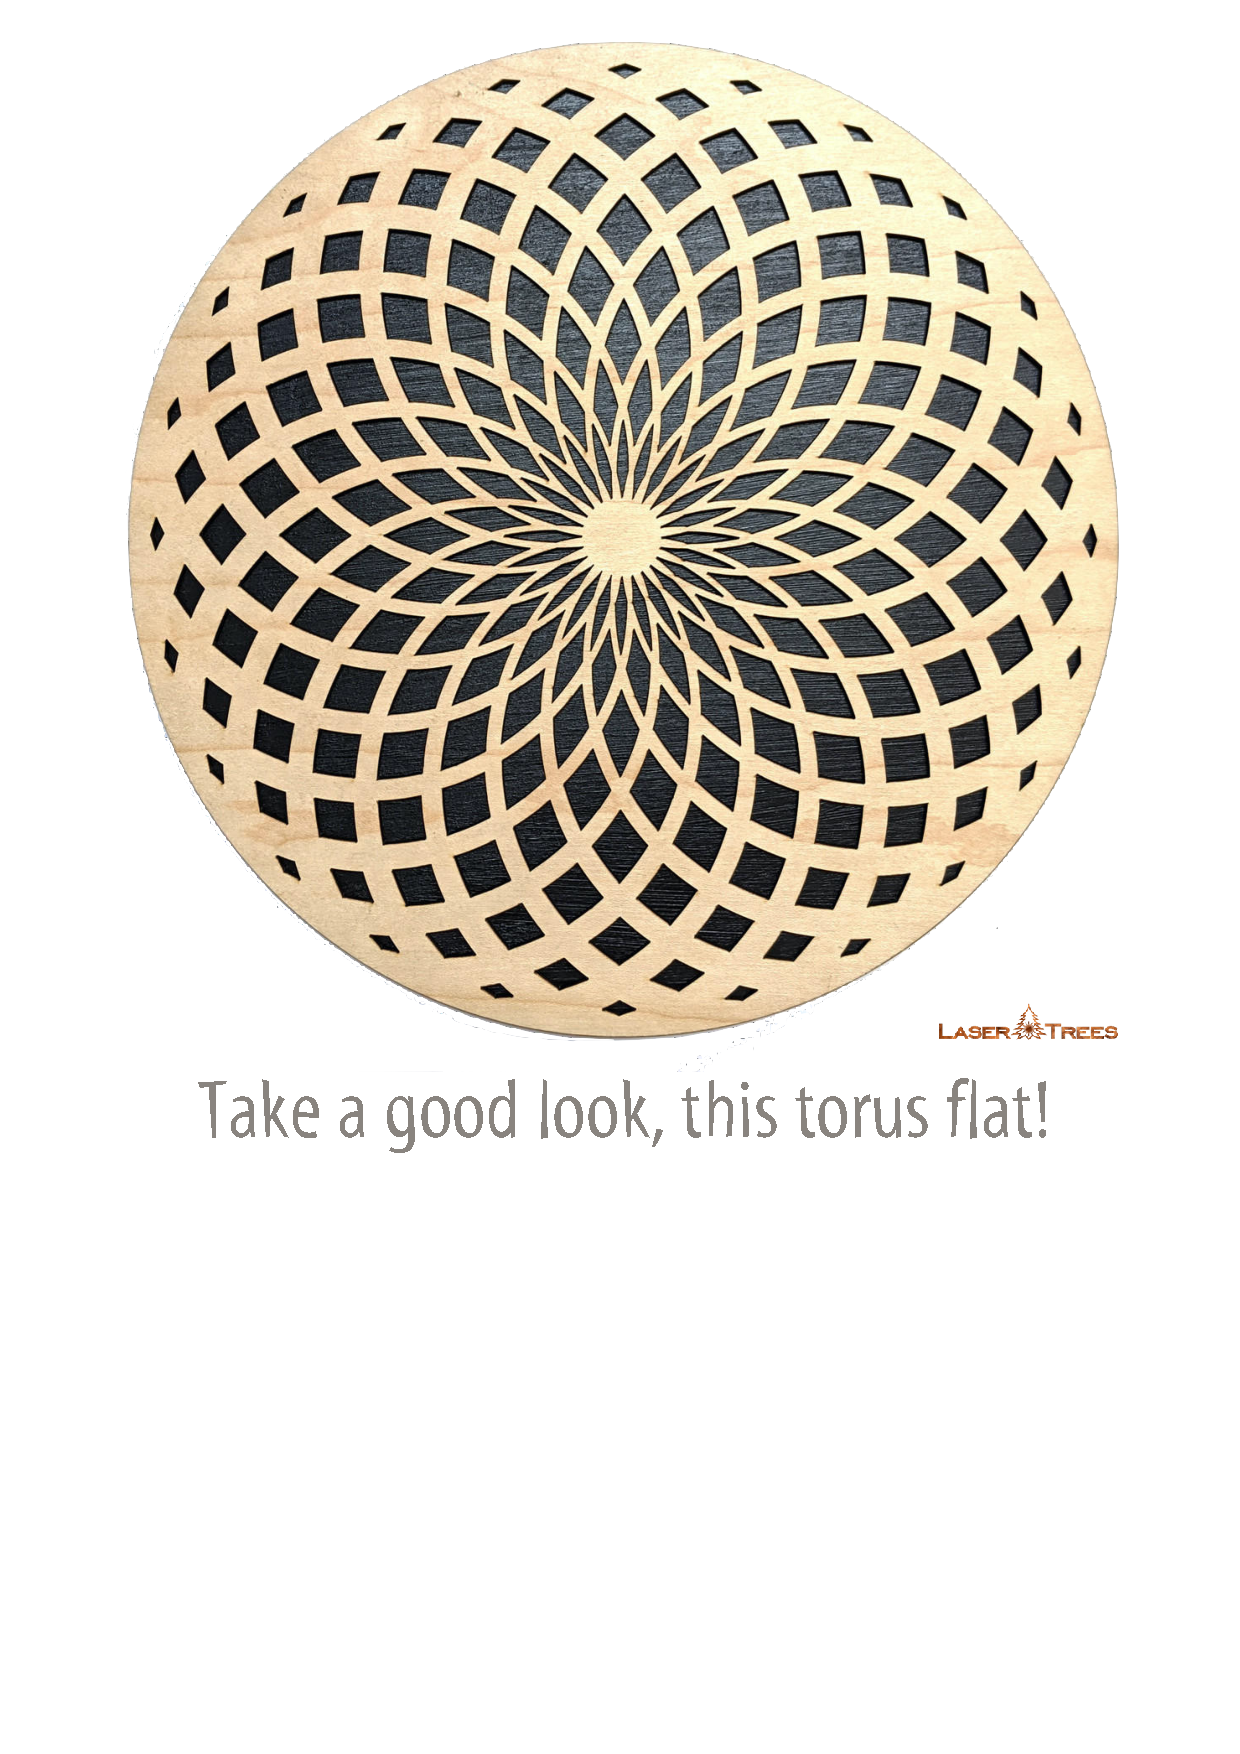
\includegraphics[width=.66\textwidth]{Figures/Torus.pdf}}
